\chapter{A Theoretical Model for The Spatial Organisation of CENP-A Nucleosomes}
\section{Introduction}

The centromere identity is primarily epigenetically determined by the histone H3 variant CENP-A in organisms with regional centromeres \citep{Warburton1997ImmunolocalizationCentromeres, Vafa1997ChromatinPlate, Earnshaw1985ThreeChromosome, Liu2006MappingCells, Regnier2005CENP-ABubR1, Heun2006, Mendiburo2011, Barnhart2011, Logsdon2015, Logsdon2019}. Contrary to the epigenetic nature, the chromosomal position of a centromere is inherited over generations of cells with astonishing fidelity and only changes if viewed from an evolutionary timescale \citep{Amor2004HumanProgress, Murphy2005DynamicsMaps}. This implies the existence of strategies ensuring the propagation, maintenance and specificity of CENP-A at centromeres. Indeed, various delicate molecular mechanisms conserved across species have been found. 

DNA replication during the S phase inevitably dilutes the number of CENP-A nucleosomes in one chromosome at least by half, where full conservation of old CENP-A is assumed. Therefore, the propagation of CENP-A nucleosomes over generations relies on the deposition of new CENP-A into the chromatin. A conserved positive feedback mechanism has emerged across different species, where old CENP-A is read by proteins that can recruit the CENP-A specific chaperon to deposit new CENP-A \citep{Stirpe2022, McKinley2015}. In vertebrates, CENP-A binds the CCAN protein CENP-C and together they recruit the Mis18 complex, consisting of Mis18$\alpha$, Mis18$\beta$ and Mis18BP1 \citep{Westhorpe2015AMaintenance, Moree2011CENP-CAssembly, Dambacher2012CENP-CChromatin, French2017XenopusAssembly, Wang2014MitoticHJURP, Pan2019MechanismLicensing}. The CENP-A chaperon HJURP bearing CENP-A-H4 heterodimer is then targeted to the centromere by the Mis18 complex \citep{Foltz2009, Dunleavy2009}. CENP-B, the centromeric protein that binds the 17-bp DNA motif CENP-B box, is reported to reinforce this process by stabilising CENP-C \citep{Fachinetti2015, Hoffmann2020, Chardon2022CENP-B-mediatedCentromeres, Masumoto1989ASatellite., Suzuki2004CENP-BLocalization} and is believed to be the 'safety net' for the positive feedback loop \citep{Berg2020}. Similarly, in fission yeast, its Mis18 complex, composed of Mis16, Mis18 and Eic1, and the CENP-A chaperon Scm3 are required for the assembly of its CENP-A ortholog Cnp1 at the centromere \citep{Pidoux2009FissionChromatin, Hayashi2004Mis16Centromeres, Williams2009FissionChromatin}, albeit the requirement for Cnp3, the fission yeast CENP-C, is not conserved \citep{Subramanian2014Eic1Assembly}. Mis18 complex and HJURP orthologs are not found in \textit{Drosophila}. But their functions are combined in one single protein CAL1, which possesses the CENP-A chaperon activity and can self-target to the centromere by interacting with CENP-C and \textit{Drosophila} CENP-A CID \citep{Chen2014, MedinaPritchard2020, Phansalkar2012EvolutionaryDrosophila, Roure2019, Schittenhelm2010}. Additional factors are required for CID deposition in this system, including the FACT complex \citep{Chen2015EstablishmentTranscription} and CAF1 \citep{Furuyama2006Chaperone-mediatedVitro, Boltengagen2016AMelanogaster}. Even in point centromere species budding yeast, whose centromeres are determined genetically, this mechanism is partially conserved. The CBF3 complex recognises the centromeric sequence CDEIII and recruits the chaperon Scm3 to deposit the CENP-A ortholog Cse4 \citep{Camahort2007Scm3Kinetochore, Guan2021StructuralFormation, Cho2011Ndc10Yeast, Mizuguchi2007NonhistoneNucleosomes, Zhou2011StructuralScm3, Meluh1998Cse4pCerevisiae}. Although the exact timing might range from late M to early G1 phase, a common feature of CENP-A deposition shared by various species is that it happens outside the S phase, unlike canonical histone proteins \citep{Fukagawa2014, McKinley2015TheFunction, Stirpe2022}. Consistent with this feature, in vertebrates, the centromeric localisation of HJURP and Mis18BP1 is prevented by CDK1/2-dependent phosphorylation, whose activity is elevated in mitosis and reduced in interphase \citep{Silva2012, Spiller2017MolecularDeposition, Stankovic2017}. The deposition machinery is further regulated by PLK1, which phosphorylates Mis18BP1 and promotes its localisation to the centromere \citep{McKinley2014Polo-likeCentromeres}. Apart from the positive feedback loop and phospho-regulation, proper deposition of CENP-A requires centromeric transcription \citep{Bergmann2012EpigeneticFunction, Catania2015SequenceChromatin, Cardinale2009HierarchicalModifier, Choi2011IdentificationCentromeres, Nakano2008InactivationModifiers, Zhu2018HistoneChromosomes}. It is reasoned that transcription facilitates new CENP-A deposition by evicting embedded non-CENP-A nucleosomes \citep{Chen2015EstablishmentTranscription, Choi2011IdentificationCentromeres, Bobkov2018, Bergmann2012EpigeneticFunction, Bobkov2020, Choi2017TheH3, Prasad2011NewCentromeres}. 

Similar to other epigenetic marks, the maintenance of CENP-A nucleosomes is challenged by chromatin remodelling activities such as replication and transcription. Yet, CENP-A possesses unusual stability that it does not turn over once incorporated into the chromatin \citep{Falk2015, Jansen2007, Bodor2013, Smoak2016Long-TermIdentity}. In replication, this has been attributed to the recycling of disrupted CENP-A-H4 heterodimer by HJURP interacting with MCM2 of the replication fork \citep{Zasadzinska2018, Zasadzinska2013DimerizationDeposition, Huang2015AForks} in a similar manner to the retention of canonical H3 by Asf1$\alpha$ \citep{Richet2015StructuralFork, Clement2015MCM2Fork}. This resulted in the conservative partition of existing CENP-A nucleosomes between the newly replicated sister chromatids \citep{Falk2015, Jansen2007, Bodor2013}. Due to the temporal separation of replicative dilution and new CENP-A deposition, the gaps generated are then filled by another histone H3 variant H3.3 as the placeholder \citep{Dunleavy2011H3.3Phase.}. As mentioned above, transcription can lead to the eviction of incorporated nucleosomes. The general chaperon FACT complex and Spt6 have been proposed to travel with RNA Pol II and reassemble CENP-A nucleosomes dissembled due to transcription \citep{Bobkov2020, Jeronimo2019HistoneModifications, Kato2013Spt6H3, Boltengagen2016AMelanogaster}.

Counter-intuitively, the majority of CENP-A nucleosomes are localised on chromosome arms \citep{Bodor2014}. This could be due to the random deposition of CENP-A caused by the large quantity and the promiscuity to general histone chaperons. Nevertheless, the centromeric enrichment is still over 50-fold higher than arms \citep{Bodor2014}. Apart from the isolation of CENP-A deposition from canonical histone proteins mentioned above, nucleosome eviction by replication, gene expression regulation and PTMs are used to improve the specificity of CENP-A at the centromere. Replication is the main mechanism to remove ectopic CENP-A nucleosomes \citep{Nechemia-Arbely2019, Wang2021PhosphorylationCycle}, with the centromeric ones being proposed to be protected by the CCAN \citep{Nechemia-Arbely2019}. In human and fission yeast cells, CENP-A transcription coincides with their respective deposition timings \citep{Shelby1997AssemblySites, Takahashi2000RequirementYeast, Aristizabal-Corrales2019CellFormation}. Moreover, it has been observed that the expression of CENP-A outside the normal time window would lead to ectopic incorporation in different organisms \citep{Aristizabal-Corrales2019CellFormation, Heun2006, Tomonaga2005CentromereAneuploidy, Au2008AlteredCerevisiae, Olszak2011, McGovern2012CentromereCancer, Athwal2015CENP-ACells, Shrestha2021, Moreno-Moreno2019TheCycle}. Among the various  PTM-based mechanisms for regulating CENP-A localisation, ubiquitin-mediated protein degradation is the most common one \citep{Stirpe2022}. In human \citep{Maehara2010CENP-AMitoses, Lomonte2001DegradationICP0}, \textit{Drosophila} \citep{Moreno-Moreno2019TheCycle, Bade2014TheManner} and budding yeast \citep{Ranjitkar2010AnDomain, Au2013AProteolysis, Mishra2015Pat1Ubiquitination, Zhou2021MolecularPsh1} cells, ubiquitination has been reported to remove CENP-A outside the centromeric regions. 

Despite that extensive studies have been conducted on the molecular biology of centromere specification and propagation, our understanding of the system is compromised due to the absence of a theoretical model. The different enrichment of CENP-A nucleosomes at centromeres and arms implicated the existence of two stable equilibrium states, or bi-stability, in the system. Positive feedback is known for its capability to generate bi-stability in biological systems \citep{Mitrophanov2008PositiveSystems, Ferrell2013FeedbackCycle}. It is tempting to hypothesise that the molecular mechanism of CENP-A deposition is sufficient to explain the difference in enrichment between centromeres and arms. Yet, the signal amplifier, or 'all or nothing', nature of positive feedback loops contrasts the low density of CENP-A nucleosomes at centromeres, where they only account for about 1 in 25 nucleosomes \citep{Bodor2014, Schittenhelm2010}. CENP-A further possesses intriguing features in terms of spatial localisation on the chromatin. Rather than distributed homogeneously, the CENP-A nucleosomes are visualised as distinct clusters on an extended chromatin fibre \citep{Blower2002ConservedHumans, Dunleavy2011H3.3Phase., Kyriacou2018}. It would be interesting to understand the mechanism behind this pattern formation. Therefore, this project aims to build a theoretical model describing the dynamics and spatial patterns of CENP-A, with the expectation to recapitulate the key characteristics of the system, including bi-stability, low density at the higher steady state and the maintenance of island patterns. 

\nomenclature{CENP}{CENtromere Protein}
\nomenclature{CCAN}{Constitutive Centromere Associated Network}
\nomenclature{HJURP}{Holliday JUnction Recognition Protein}
\nomenclature{CID}{Centromere IDentifier}
\nomenclature{FACT}{Facilitates Chromatin TranscripTion}
 
\section{Methods}
\subsection{The model}

Inspired by the classic theoretical model for epigenetics \citep{Dodd2007, Micheelsen2010TheoryLandscapes}, we decided to use a CA-like, 1D, rule-based stochastic model for the CENP-A system. As a starting point, we developed a basic model, where the molecular knowledge of CENP-A propagation and maintenance is described in its simplest manner. The assumptions used for the basic model are as follows: 

(1) A certain number of sequentially placed nucleosomes composed of either canonical H3 or CENP-A nucleosomes was considered to represent the centromere. Because the lengths of centromeres vary largely among species and even between different chromosomes in the same species, we did not set a fixed value for the number of nucleosomes. As will be shown in the later section, this variable only provides a minor effect on the model's behaviours. Periodic boundary conditions were used to avoid potential artefacts from boundaries. 

(2) At each time step, CENP-A nucleosomes are first replenished and then diluted (Figure~\ref{fig:basicmodelschematics}B). This is because CENP-A is deposited at the interphase while diluted at the S phase in most species. The two processes will be referred to as 'replenishment' and 'dilution' in the following texts for convenience. We assume no loss of CENP-A except replicative dilution as the ultra-low turnover rate of CENP-A nucleosomes mentioned above. 

(3) For replenishment, H3 nucleosomes were converted to CENP-A nucleosomes because of pre-existing CNEP-A nucleosomes in proximity (Figure~\ref{fig:basicmodelschematics}A). Notably, the positive feedback of CENP-A deposition was simplified as its local self-promoting property in this case. The detailed algorithm of this process will be described in the following implementation sub-section. 

(4) For dilution, CENP-A nucleosomes were assumed to be randomly distributed to daughter centromeres as observed in wet-lab experiments (Figure~\ref{fig:basicmodelschematics}A). 

\begin{figure}[htbp]
  \centering
  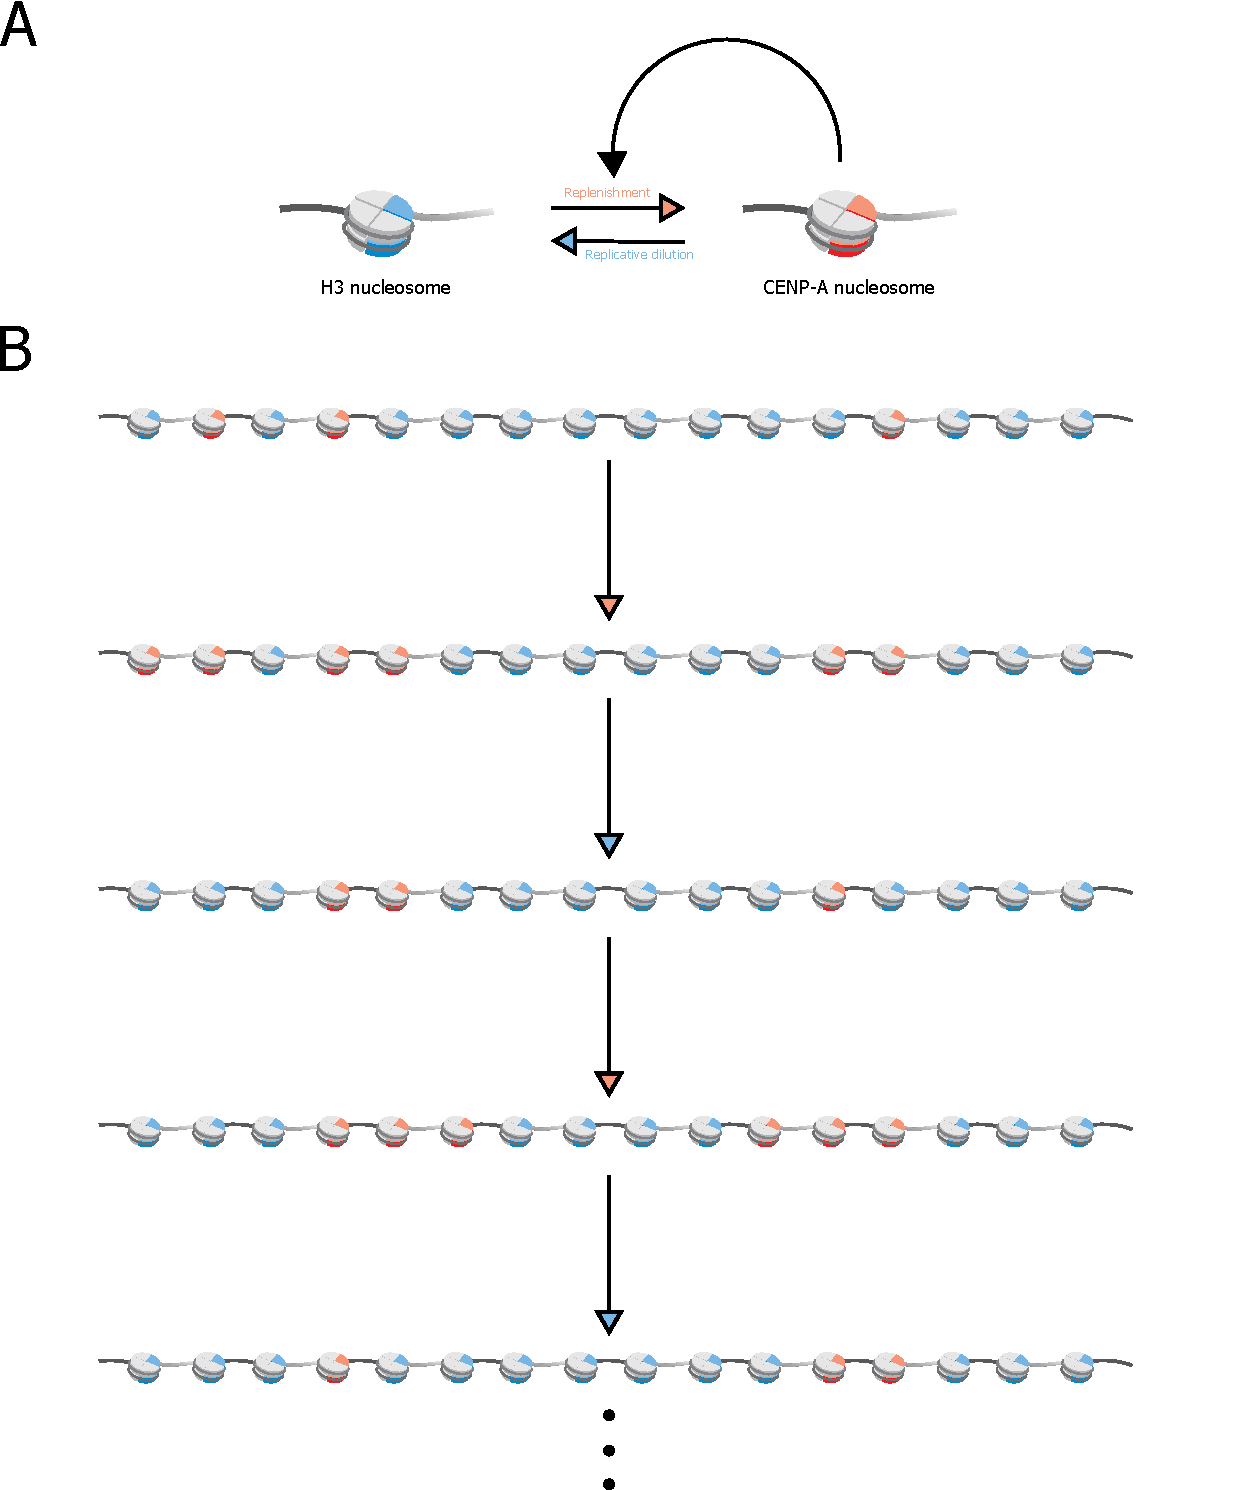
\includegraphics[width=0.9\textwidth]{chapter2/figures/the model.pdf}
  \caption[Schematics of the basic model]{Schematics of the basic model. (A) Schematics of the interchange between CENP-A and H3 nucleosomes. CENP-A nucleosomes are converted to H3 nucleosomes due to replicative dilution. H3 nucleosomes are converted to CENP-A nucleosomes by replenishment, where pre-existing CENP-A nucleosome facilitates the conversion of H3 nucleosomes locally. (B) An example of the evolution of the basic model. The array of nucleosomes undergoes replenishment and dilution at each cell cycle. }
  \label{fig:basicmodelschematics}
\end{figure}

\nomenclature{CA}{Cellular Automata}
\nomenclature{1D}{one-Dimensional}

\subsection{Implementation}

The model describes the centromere as a 1D array of a certain number, denoted by $NN$, of cells with two states, either 1, representing the CENP-A nucleosome or 0, representing the H3 nucleosome.

\subsubsection{Initialisation}

To unbiasedly initialize such an array, a stochastic approach is used. a 1D array of 0 was first created. Each 0 in the array then has a probability of the arbitrary initial CENP-A density, denoted by $\rho_{0}$, to be converted to 1. A typical array was exemplified in Figure~\ref{fig:array}. The density and spatial pattern of CENP-A are used as read-outs of the state of the  array. Density is calculated by dividing the sum of the array, which equals the number of 1s in the array, by the length of the array. As a mimicry of CENP-A imaging data from biological experiments, spatial pattern is visualized by plotting the array with 1 as white and 0 as black. \\

\begin{figure}[htbp]
  \centering
  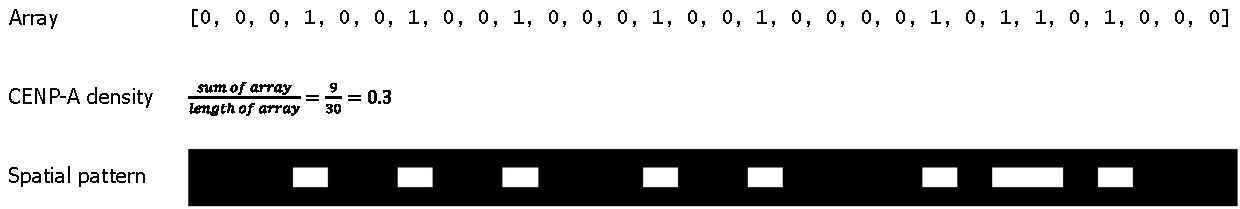
\includegraphics[width=0.9\textwidth]{chapter2/figures/the array.pdf}
  \caption[The implementation of the basic model]{The implementation of the basic model. The centromere is described as a finite 1D array composed of only 0 and 1, with 0 representing the H3 nucleosome and 1 representing the CENP-A nucleosome. The density of CENP-A is calculated by dividing the sum of the array by the length, or the number of cells, of the array. The spatial pattern of CENP-A distribution is visualised by colouring 1 as white and 0 as black. }
  \label{fig:array}
\end{figure}

\subsubsection{Replenishment}

As with other CA models, our model updates the state of a cell by a state-transition function that reads the states of neighbour cells. To describe the replenishment, where new CENP-A nucleosomes replace H3 nucleosomes due to pre-existing CENP-A and the CENP-A nucleosomes do not turn over, we set the state-transition function as such: 
\begin{align*}
    & P_{0\rightarrow 1}=\alpha\sum_{i=-n}^{n} x_if_i \\
    & P_{1\rightarrow 0}=0 
\end{align*}
where $\alpha$ is an arbitrary parameter denoting the loading efficiency, $n$ denotes the size of the neighbourhood, $x$ is the state of the cell $i$ and $f$ is the weight function, which is a Gaussian function with a mean of 0 and a standard deviation of n/3 ($f\sim Gaussian(\mu=0, \sigma=\frac{n}{3}$) used to model the assumption that the probability of interaction decreases with physical distance. 

To enable more flexibility of replenishment, we allowed it to happen multiple rounds before dilution. The number of rounds was denoted by $rr$. 

\subsubsection{Dilution}

Ideally, one array should be divided into two daughter arrays during each dilution event. Yet, the number of arrays would grow exponentially with the simulation steps, as would the computational time required. To simulate the evolution of the array for more steps, only one of the daughter arrays was tracked. Hence, replicative dilution is modelled by the process where each 1 in the array has a probability of 0.5 to be converted to 0, which leads to the following state-transition function: 
\begin{align*}
    & P_{0\rightarrow 1}=0 \\
    & P_{1\rightarrow 0}=0.5
\end{align*}
The parameters of the basic model were summarised in Table~\ref{tab:parameters}. \\

\begin{table}[htbp]
\centering
\caption{The parameters of the basic model}
\label{tab:parameters}
\begin{tabular}{cl}
\hline
\textbf{Parameters} & \multicolumn{1}{c}{\textbf{Description}} \\ \hline
$NN$                  & The number of nucleosomes                \\
$\rho_{0}$               & The initial density of CENP-A            \\
$\alpha$               & The  loading efficiency                  \\
$n$                   & The size of neighbourhood                \\
$rr$                  & The number of replenishment rounds      \\ \hline
\end{tabular}
\end{table}

\section{Results}
\subsection{The basic model exhibits two types of behaviour}

We started by experimenting with different combinations of parameters and classifying behaviours of the basic model based on CENP-A density evolution maps (Figure~\ref{fig:modelBehaviour}A and B left). A density evolution map presents how CENP-A density changes over time. In general, two types of behaviour were observed. First, the density eventually
reaches 0 (Figure~\ref{fig:modelBehaviour}A). Due to the fact that new CENP-A nucleosomes require old CENP-A nucleosomes to be recruited, once the density reaches 0, it will stay at 0. We named this type of behaviour ‘dead’. The second type is where CENP-A density is fluctuating around a value less than 0.5 after a number of generations (Figure~\ref{fig:modelBehaviour}B). We called this type of behaviour ‘stabilized’. The maximal value of density cannot be greater than 0.5 because we update the array by first replenishing and then diluting it. Then we sought to visualise the evolution of the CENP-A spatial pattern of the two behaviours by stacking spatial patterns according to generation. We termed this plot spatial pattern kymograph (Figure~\ref{fig:modelBehaviour}A and B right). For the ‘dead’ type behaviour, CENP-A nucleosomes formed inheritable aggregates, or islands, which could diverge or be combined. But all the islands vanished eventually. For the ‘stabilized’ behaviour, the islands could be seen in the first several time steps. After that, the islands joined each other and formed random-like distribution of CENP-A. Given the auto-amplification property of CENP-A deposition, the existence of ‘stabilized’ behaviours, where CENP-A density can be stabilised before saturation, is surprising. We reasoned that this is because as the density of CENP-A nucleosome increases, the number of H3 nucleosomes decreases, leading to a reduced room for new CENP-A to be deposited. This counteracts auto-amplification and results in a steady state. 

We next attempted to systematically view how model behaviours change with parameters. Due to the predictable positive effect on the CENP-A density of $rr$, I fixed it and ran simulations with different combinations of the loading efficiency $\alpha$ ranging from 0 to 1 with a step size of 0.02 and the range of local deposition $\sigma$ ranging from 0 to 10 with a step size of 0.2. Each simulation was conducted for 500 time steps and assigned to either ‘dead’ or ‘stabilised’ type based on whether the average density of the first 100 time steps is less or greater than the last 100 time steps. The result showed that the two behaviours fall into two separate phases (Figure~\ref{fig:modelBehaviour}C). Both $\alpha$ and $\sigma$ were positively correlated to the ‘stabilized’ behaviour. Interestingly, the boundary between the two phases can roughly be described by a reciprocal function.

To quantitatively visualise the transition from the 'dead' to 'stabilised' behaviour, we wanted to investigate how the asymptotic CENP-A nucleosome density responds to changes in $\alpha$. Therefore, I ran long simulations (10,000 time steps) of the model with $\alpha$ ranging from 0.4 to 1 with a step size of 0.01. The average of the last 2,000 time steps was used as the read-out of the asymptotic density. As shown in Figure~\ref{fig:modelBehaviour}D, the asymptotic density stayed at 0 and does not change with $\alpha$ at the beginning. After around $\alpha$=0.5, it started to increase according to $\alpha$ and formed a concave curve saturating at above 0.4. To better quantify the transition, I decided to simulate with longer time steps and finer resolution of $\alpha$. I then conducted simulations of 100,000 time steps and $\alpha$ ranging from 0.5 to 0.53 with a step size of 0.003. The result was nearly identical to the 10,000-step simulation with data points roughly on the same curve (Figure~\ref{fig:modelBehaviour}D). 

\begin{figure}[htbp]
  \centering
  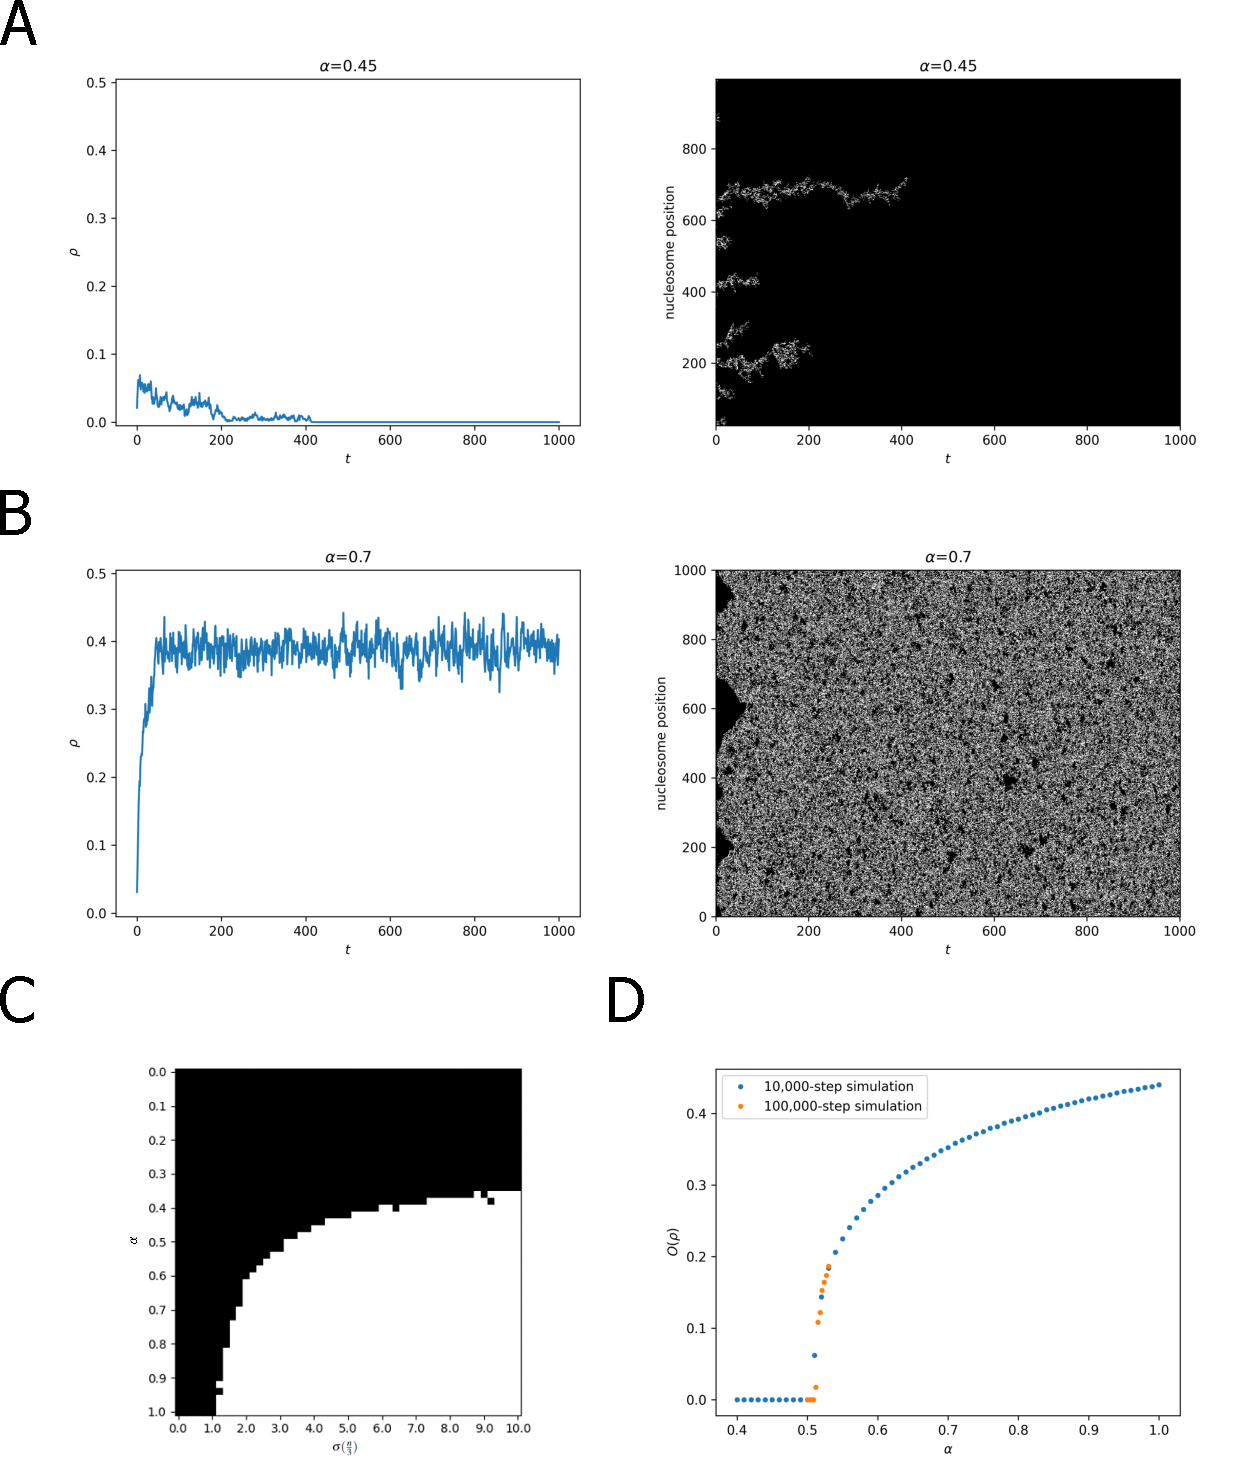
\includegraphics[width=0.9\textwidth]{chapter2/figures/model_behaviour.pdf}
  \caption[Typical behaviours of the basic model.]{Typical behaviours of the basic model. The simulations were conducted at $NN$=1000, $\rho_{0}$=0.02, $\sigma$=3, $rr$=3 if not otherwise stated. (A) The density evolution map and spatial pattern kymographs of a representative ‘dead’ behaviour ($\alpha$=0.45). (B) The density evolution map and spatial pattern kymographs of a representative ‘stabilised’ behaviour ($\alpha$=0.7). (C) Phase diagram of the model behaviour as a function of $\alpha$ and $\sigma$. Black represents the ‘dead’ behaviour and white represents the ‘stabilised’ behaviour for a specific parameter set. (D) Asymptotic density as a function of $\alpha$. 10 simulations were run for 10,000 (blue) or 100,000 time steps (orange) and the average density of the last 2,000 time steps was plotted as the asymptotic density. }
  \label{fig:modelBehaviour}
\end{figure}

We further tested if other factors might change the behaviours of the basic model. Generally, different simulations with the same parameter set generated qualitatively similar results (Figure~\ref{fig:parameterTest}A), suggesting that stochasticity is not important in determining the model behaviour. The number of nucleosomes also had little effect on the asymptotic density, though the smaller number showed a higher noise (Figure~\ref{fig:parameterTest}B). The initial value matters if the system has more than one steady state. To test it, I simulated the model from various initial densities. However, they all approached the same asymptotic value eventually (Figure~\ref{fig:parameterTest}C), indicating the model is likely to possess only one steady state. Note that the curves of high initial density appeared to be non-smooth in the first time step. This is because, independent of the initial value, they were all reduced to 0.5 after the first time step due to saturation. 

\begin{figure}[htbp]
  \centering
  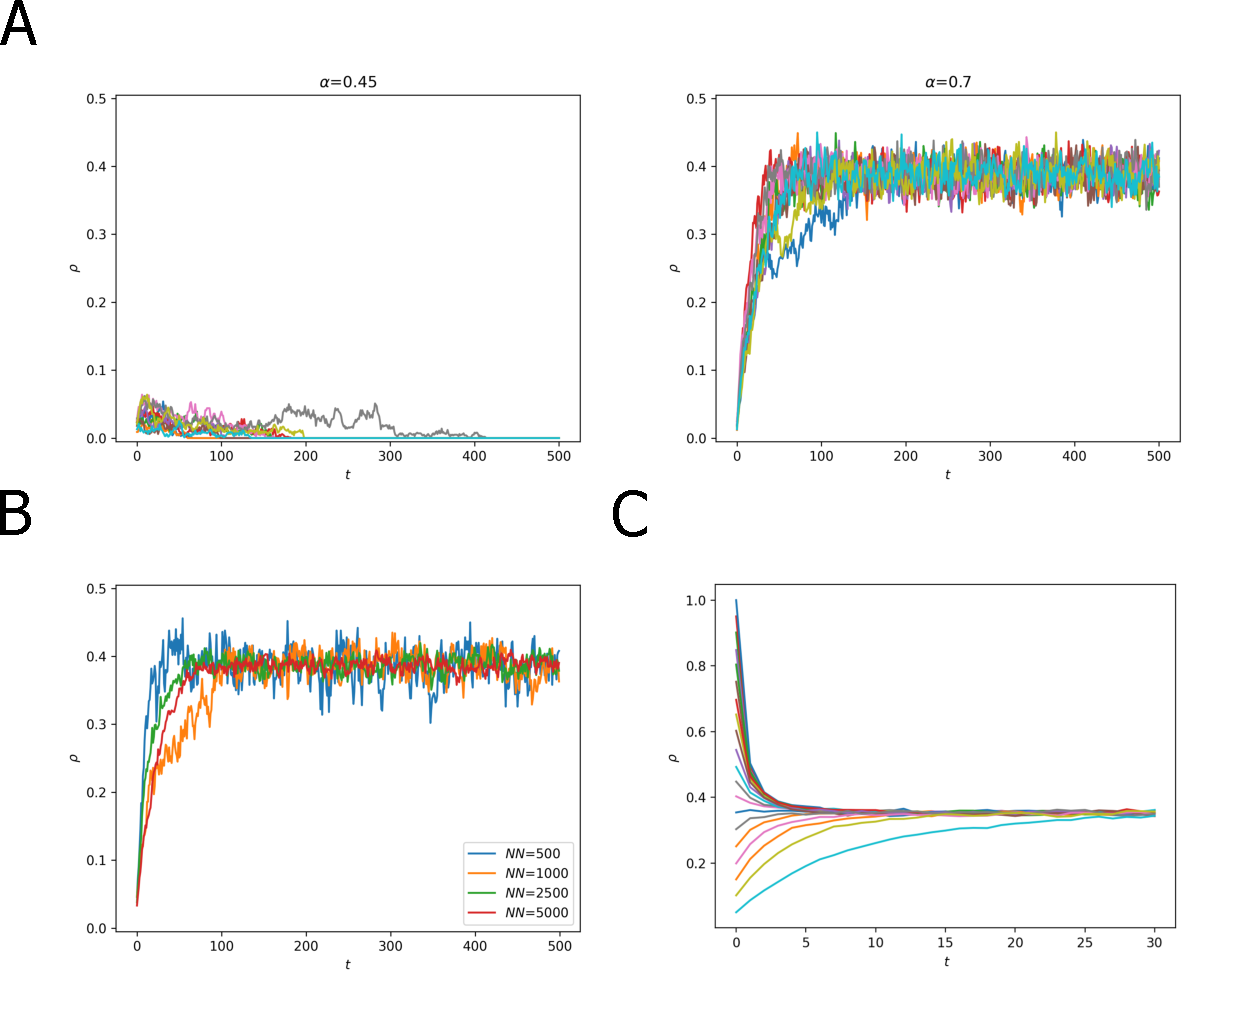
\includegraphics[width=0.9\textwidth]{chapter2/figures/parameter_test.pdf}
  \caption[The model behaviours are insensitive to stochasticity, nucleosome number and initial density]{The model behaviours are insensitive to stochasticity, nucleosome number and initial density. The simulations were conducted at $NN$=1000, $\rho_{0}$=0.02, $\alpha$=0.7, $\sigma$=3, $rr$=3 if not otherwise stated. (A) The density evolution maps of different simulations of the representative ‘dead’ or 'stabilised' behaviour. 10 simulations were conducted for each behaviour, shown in different colours. (B) The density evolution map of the representative ‘stabilised' behaviour with different $NN$s. (C) The density evolution map of the representative ‘stabilised' behaviour with different $\rho_{0}$s. For each $\rho_{0}$, 100 simulations with $NN$=200 were conducted for 30 time steps. Each colour represents the average of 100 simulations. }
  \label{fig:parameterTest}
\end{figure}

In summary, the basic model (Figure~\ref{fig:basicmodelschematics}A) has two possible outcomes, with either all CENP-A nucleosomes being eventually lost or the density being maintained at a value much higher than that of the real biological systems. Moreover, in the second case, CENP-A nucleosome distribution is obviously different from the ‘islands’ pattern seen in extended chromatin experiments. Hence, we concluded that local deposition only is not sufficient to recapitulate the CENP-A dynamics \textit{in vivo}.

\subsection{Mean-field approximation is able to qualitatively explain the simulation results}

By simulating the old model and analyzing the results, we had a qualitative view of the basic model. To analyze the model
quantitatively, I wanted to apply analytical methods. Given the similarity between our model to CA, I chose mean-field
approximation as suggested by \citep{Sayama2013IntroductionSystems}. Instead of specific states of the system, mean-field approximation re-describes the dynamics of the system as how individual cells interact with the ’average state’ and how the ’average state’ itself changes over time. 

As mentioned above, the CENP-A nucleosome was expressed as cell state 1 whereas the H3 nucleosome was expressed as cell state 0 for the convenience of calculation. After applying mean-field approximation, the system now only has one state variable $\rho_{t}$, the density of 1s at time step t. To monitor its evolution, one needs to enumerate all possible scenarios of individual CA cells interacting with $\rho_{t}$ and their probabilities (Table~\ref{tab:MFAscenariosBasic}). Here, I started with one round of replenishment for simplicity. I identified 4 possible scenarios:

\begin{table}[htbp]
\centering
\caption{Possible scenarios of an individual cell in a one-round replenishment event of the basic model}
\label{tab:MFAscenariosBasic}
\begin{tabular}{cccc}
\hline
\textbf{Scenario} & \textbf{Current state} & \textbf{Updated state} & \textbf{Probability} \\ \hline
(1) & 1                        & 0                      & 0                    \\
(2) & 1                        & 1                      & $\rho_{t}$                    \\
(3) & 0                        & 1                      & $(1 - \rho_{t})P_{0\rightarrow 1}(\rho_{t})$     \\
(4) & 0                        & 0                      & $(1 - \rho_{t})(1 - P_{0\rightarrow 1}(\rho_{t}))$ \\ \hline
\end{tabular}
\end{table}


(1) The cell state is 1 at time step t and will become 0 at time step t+1. The probability of finding a cell of 1 is simply $\rho_{t}$. But due to the assumption that CENP-A nucleosomes are not removed from the chromatin other than during dilution, the probability of this scenario is $\rho_{t} \times 0 = 0$. 

(2) The cell state is 1 at time step t and will stay 1 at time step t+1. For the same reason as above, the probability of this scenario is $\rho_{t} \times 1 = \rho_{t}$. 

(3) The cell state is 0 at time step t and will become 1 at time step t+1. Since the binary nature of cell state, the probability of finding a cell of 0 is $1 - \rho_{t}$. Then for this scenario to happen, one needs to consider the 0 to 1 state-transition function at $\rho_{t}$, which was denoted as $P_{0\rightarrow 1}(\rho_{t})$. Therefore, the probability of this scenario can be expressed as $(1 - \rho_{t})P_{0\rightarrow 1}(\rho_{t})$. 

(4) The cell state is 0 at time step t and will stay 0 at time step t+1. The occurrence of this scenario is equivalent to 
the fact that scenario (3) does not happen. Hence the probability of this scenario can be expressed as $(1 - \rho_{t})(1 - P_{0\rightarrow 1}(\rho_{t}))$.


After one round of replenishment, the density 1s equals the sum of the updated state of each scenario weighted by its respective probability. Hence, the one-round replenish function R can be written as:
\begin{equation}\label{eq:1}
\begin{split}
                R(\rho_{t})
                &= 0 \times 0 + 1 \times \rho_{t} + 1 \times (1 - \rho_{t})P_{0\rightarrow 1}(\rho_{t}) \\
                & + 0 \times (1 - \rho_{t})(1 - P_{0\rightarrow 1}(\rho_{t})) \\
                &=\rho_{t} + (1 - \rho_{t})P_{0\rightarrow 1}(\rho_{t})
\end{split}
\end{equation}
With the consideration that there is always a cell of 0 in the middle (position 0), the 0 to 1 state-transition function at $\rho_{t}$, $P_{0\rightarrow 1}(\rho_{t})$, can be calculated as follows: 
\begin{equation}\label{eq:2}
\begin{split}
                P_{0\rightarrow 1}(\rho_{t})
                &=\alpha(\rho_{t}f(-n)+\rho_{t}f(-n+1)\\
                &\quad+\ldots+0\cdot f(0)+\ldots+\\
                &\quad \rho_{t}f(n-1)+\rho_{t}f(n))\\
                &=\alpha(1-f(0))\rho_{t}
\end{split}
\end{equation}
Substitute $P_{0\rightarrow 1}(\rho_{t})$ in Equation~\ref{eq:1} with Equation~\ref{eq:2}, one can obtain:
\begin{equation}\label{eq:3}
                R(\rho_{t}) = \rho_{t} + (1 - \rho_{t})\alpha(1 - f(0))\rho_{t}
\end{equation}
By defining a new parameter $\omega = \alpha(1 - f(0))$, Equation~\ref{eq:3} becomes:
\begin{equation}\label{eq:4}
                R(\rho_{t}) = -\omega \rho_{t}^{2} + (1 + \omega) \rho_{t}
\end{equation}
The density of 1 at the next time step t+1 can then be calculated by implementing multiple rounds of replenishment as the recursion of function R and dilution as a halving of density:
\begin{equation}\label{eq:5}
                \rho_{t+1} = \frac{R^{rr}(\rho_{t})}{2}
\end{equation}
Combining Equation~\ref{eq:4} and Equation~\ref{eq:5}, the mean-field approximation of the basic model can be expressed as:
\begin{equation}\label{eq:6}
\begin{split}
            &\rho_{t+1} = \frac{R^{rr}(\rho_{t})}{2} \\
            &R(\rho_{t}) = -\omega \rho_{t}^{2} + (1 + \omega) \rho_{t}
\end{split}
\end{equation}
where $\omega = \alpha(1 - f(0))$. 

With the mathematical formulation of the basic model, we were able to analyse how the model behaviour was determined. To identify the existence of steady states and understand their changes according to $\alpha$, I started with the iterative map, or Cobweb plot, of the mean-field approximation with $\alpha$ ranging from 0 to 1 (Figure~\ref{fig:meanFieldApproximation}A). The Cobweb plot showed $\rho_{t+1}$ as a function of $\rho_{t}$. Its intersections with $y=x$ were therefore the fixed points of the model. Their stability can be assessed by the first-order derivative $y'$ at that point. If $\lvert y' \rvert \le 1$, the fixed point is stable. As shown in the Cobweb plot, the system’s fixed point(s) depends on $\alpha$. Low $\alpha$ has only one stable fixed point at $\rho_{t}$=0 while it becomes unstable for higher $\alpha$. Meanwhile, a non-zero stable fixed point starts to appear. To systematically study the effect of $\alpha$ on the steady state(s) of the system, I constructed the bifurcation diagram, where the fixed densities were plotted as a function of $\alpha$ (Figure~\ref{fig:meanFieldApproximation}B). The bifurcation diagram indicated that the fixed density stayed at 0 and did not change with $\alpha$ at the beginning. However, after around $\alpha$=0.3, the fixed density started to become positively correlated to $\alpha$. From a mathematical point of view, the system undergoes transcritical bifurcation as $\alpha$ increases. Interestingly, contrary to the simulation results that the asymptotic density is either 0 or a much higher value, the non-zero stable fixed point by the mean-field approximation can be very close to 0. We reasoned that it might be because the systems with small fixed densities were prone to stochasticity that could lead to 0 density and they would stay at 0 once they reached there. Thus, in simulations, small fixed densities were unable to be observed. Next, I wanted to compare the predicted fixed densities by mean-field approximation with the asymptotic densities from the simulations. As shown in Figure~\ref{fig:meanFieldApproximation}C, the prediction showed a similar trend as the simulation data, albeit there were quantitative differences. Therefore, I concluded that mean-field approximation is capable of qualitatively describing the system. 

\begin{figure}[htbp]
  \centering
  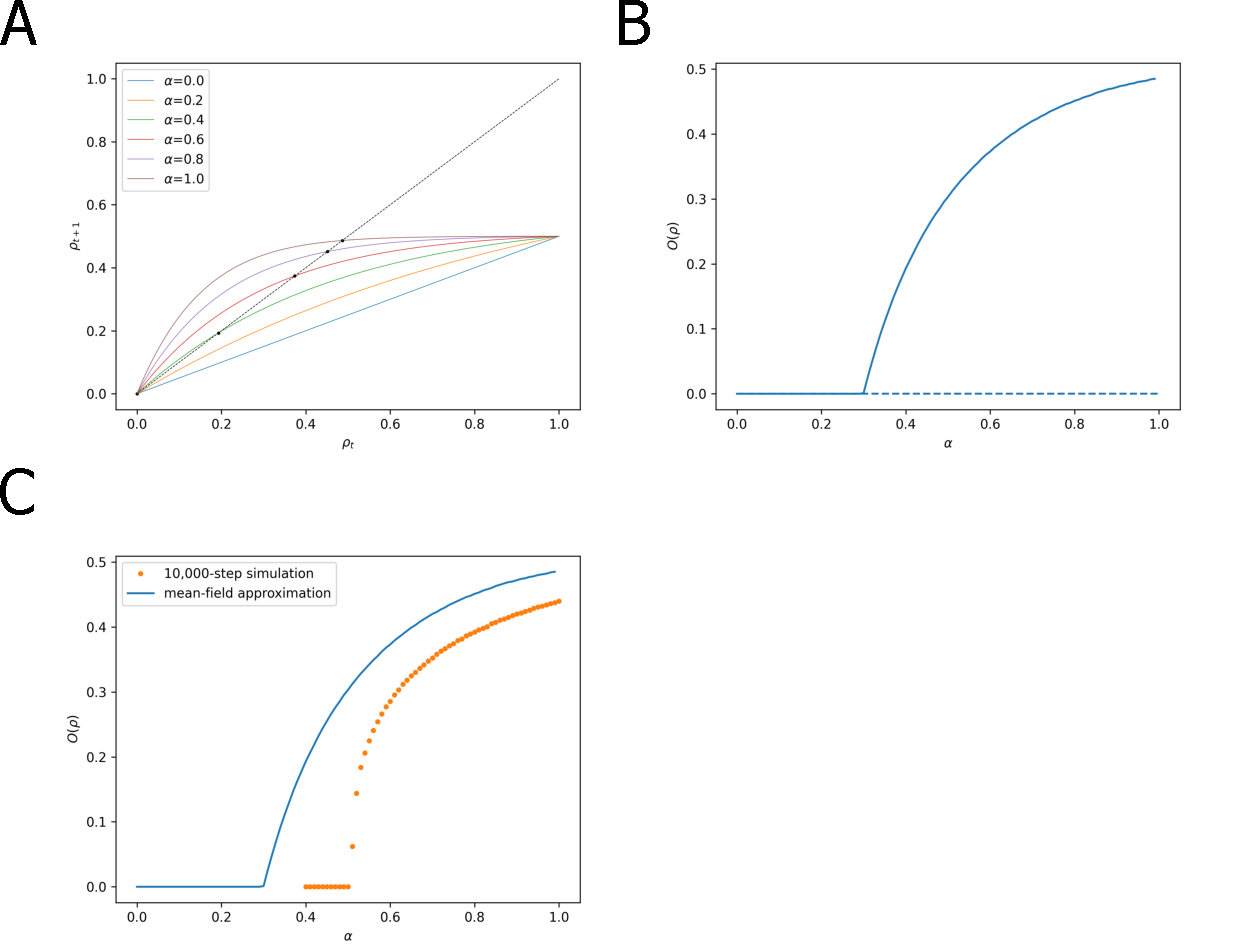
\includegraphics[width=0.9\textwidth]{chapter2/figures/mean-field_approximation.pdf}
  \caption[Mean-field approximation of the basic model]{Mean-field approximation of the basic model. $rr$=3 was used if not otherwise stated. (A) Cobweb plot of the basic model. The mean-field approximations of the basic model with different $\alpha$s were shown as coloured curves. Their intersections with $y = x$ represent fixed points, which were indicated as black dots. (B) Bifurcation diagram of the basic model. The fixed densities were plotted as a function of $\alpha$. The stable branch was shown as the solid line, whereas the unstable one was shown as the dotted line. (C) Comparison between the prediction of mean-field approximation and the simulation. The asymptotic densities were plotted as a function of $\alpha$. The stable branch of mean-field approximation was shown as the blue curve. The 10,000-step simulations were shown as orange dots.}
  \label{fig:meanFieldApproximation}
\end{figure}

\subsection{Global cooperative deposition generates bi-stability but cannot maintain the higher steady state at a low density}

As both behaviours of the basic model could not recapitulate CENP-A dynamics in real biological systems, we decided to introduce new mechanisms to the system. It is well established that non-linearity in the positive feedback loop is required for bi-stability to occur in a 1D epigenetics model \citep{Dodd2007, Micheelsen2010TheoryLandscapes, Dodd2017}. Cooperativity, the requirement of more than one copy of the protein to function, is a possible mechanism of non-linearity for our model because it has been proposed that a CENP-C dimer binds two CENP-A nucleosomes simultaneously \citep{Walstein2021}. To introduce such cooperativity, I modified the deposition rule to that two pre-existing CENP-A nucleosomes are needed for the incorporation of a new CENP-A (Figure~\ref{fig:coopSchematics}A). The probability of each possible scenario during one round of replenishment changes accordingly (Table~\ref{tab:MFAscenariosCoop}). 

\begin{table}[htbp]
\centering
\caption{Possible scenarios of an individual cell in a one-round replenishment event of the cooperative deposition model}
\label{tab:MFAscenariosCoop}
\begin{tabular}{cccc}
\hline
\textbf{Scenario} & \textbf{Current state} & \textbf{Updated state} & \textbf{Probability} \\ \hline
(1) & 1                        & 0                      & 0                    \\
(2) & 1                        & 1                      & $\rho_{t}$                    \\
(3) & 0                        & 1                      & $(1 - \rho_{t})\rho_{t}P_{0\rightarrow 1}(\rho_{t})$     \\
(4) & 0                        & 0                      & $(1 - \rho_{t})(1 - \rho_{t}P_{0\rightarrow 1}(\rho_{t}))$ \\ \hline
\end{tabular}
\end{table}

And the Mean-field approximation becomes:
\begin{equation}\label{eq:7}
\begin{split}
            &\rho_{t+1} = \frac{R^{rr}(\rho_{t})}{2} \\
            &R(\rho_{t}) = -\omega \rho_{t}^{3} + \omega \rho_{t}^{2} + \rho_{t}
\end{split}
\end{equation}
where $\omega = \alpha(1 - f(0))$. 

From the Cobweb plot, it can be seen that similar to the basic model, the curve only has one fixed point for small $\alpha$s. As $\alpha$ increases, the curvity of the function grows and results in the emergence of two additional fixed points. Analysing the slopes at the intersections indicated that the middle one is unstable whereas the other two are stable (Figure~\ref{fig:coopSchematics}B). The bifurcation diagram showed that this represents a saddle-node bifurcation (Figure~\ref{fig:coopSchematics}C). 

\begin{figure}[htbp]
  \centering
  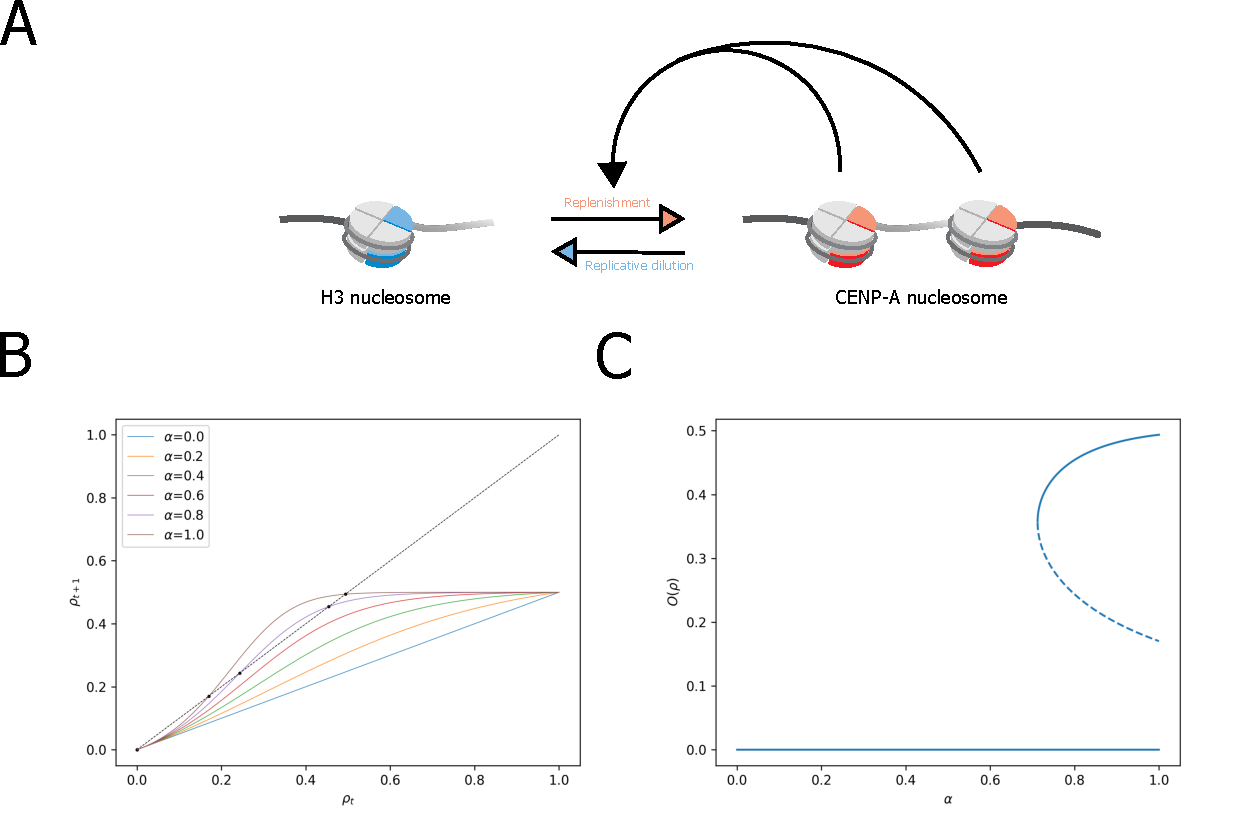
\includegraphics[width=0.9\textwidth]{chapter2/figures/cooperativity.pdf}
  \caption[The schematics and mean-field approximation of the cooperative deposition model]{The schematics and mean-field approximation of the cooperative deposition model. (A) Schematics of the cooperative deposition model. (B) Cobweb plot of the cooperative deposition model. The mean-field approximations of the cooperative deposition model with different $\alpha$s were shown as coloured curves. The fixed points were indicated as black dots. (C) Bifurcation diagram of the cooperative deposition model. The fixed densities were plotted as a function of $\alpha$. The stable branch was shown as the solid line, whereas the unstable one was shown as the dotted line.}
  \label{fig:coopSchematics}
\end{figure}

To verify the mean-field approximation, I implemented cooperativity in the simulation algorithm. On the first attempt, I kept the cooperativity local, which means both the two pre-existing CENP-A nucleosomes had to be within the neighbourhood of the nucleosome to transit. After testing various combinations of parameters, I found that the local cooperative deposition model possessed similar behaviours to the basic model in that the asymptotic density was maintained at either high values or 0, independent of the initial density $\rho_{0}$ (Figure~\ref{fig:localCoop}). Note that higher $rr$ had to be used in this case to generate the non-zero steady state. This is because the probability of depositing a new CENP-A is reduced when cooperativity is introduced. Contrary to the mean-field approximation, the local cooperative deposition model failed to generate bi-stability. However, it is in line with the conclusion by \cite{Dodd2007} that 'beyond-neighbour' interactions were required for bi-stability to occur in the 1D epigenetics model. 

\begin{figure}[htbp]
  \centering
  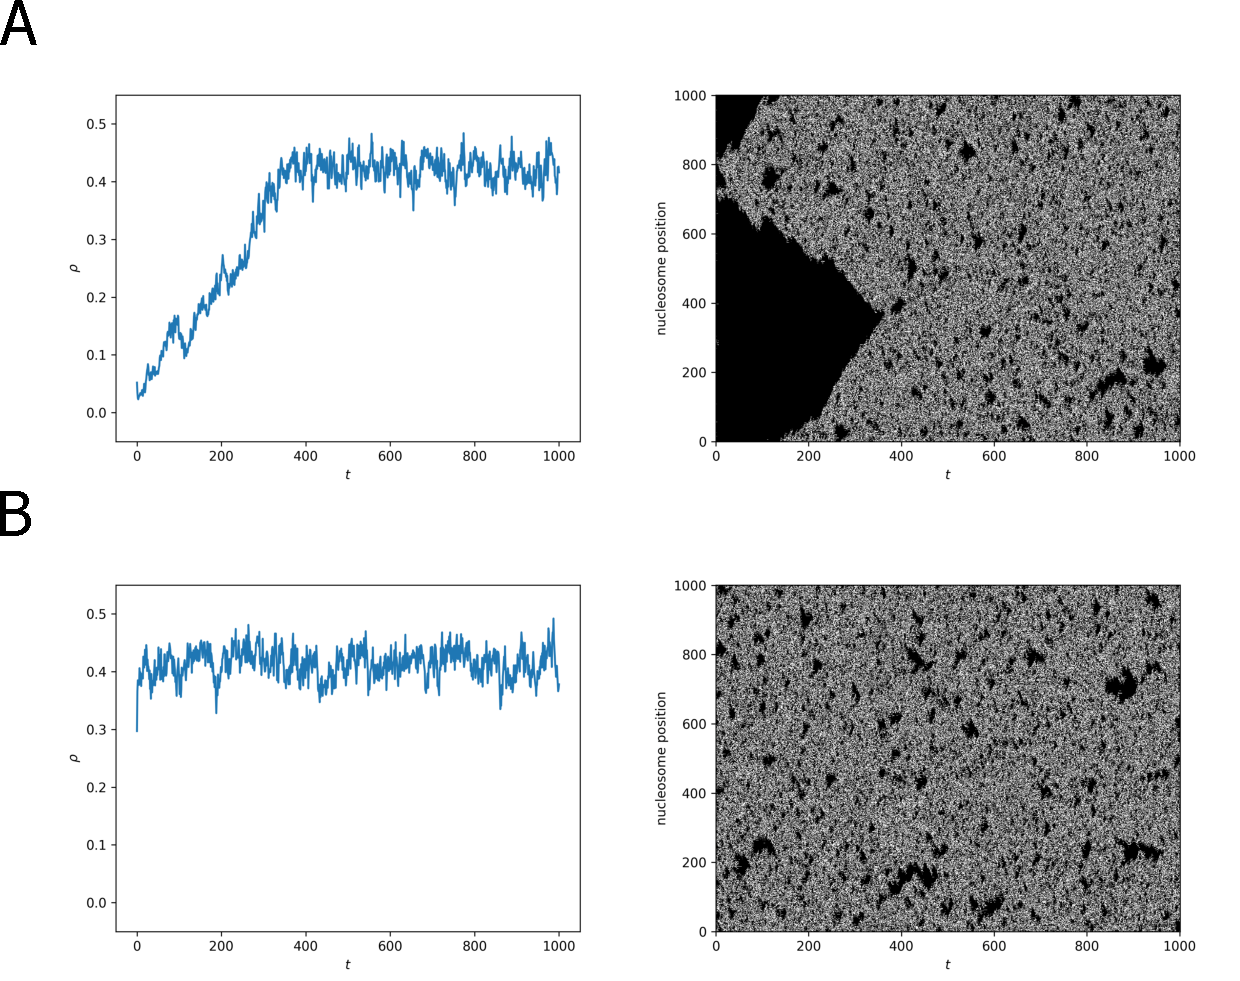
\includegraphics[width=0.9\textwidth]{chapter2/figures/local_coop.pdf}
  \caption[Local cooperative deposition could not generate bi-stability]{Local cooperative deposition could not generate bi-stability. The simulations were conducted at $NN$=1000, $\alpha$=1, $\sigma$=3, $rr$=7. (A) The density evolution map and spatial pattern kymographs of the local cooperative deposition model starting from low initial density ($\rho_{0}$=0.05). (B) The density evolution map and spatial pattern kymographs of the local cooperative deposition model starting from high initial density ($\rho_{0}$=0.3).}
  \label{fig:localCoop}
\end{figure}

Therefore, on the second attempt, I implemented global cooperativity that only one of the two pre-existing CENP-A nucleosomes was need to be within the neighbourhood while the other one could be at any position. As expected, the global cooperative model was able to exhibit bi-stability. With the same parameter set, the asymptotic density of the model could be either 0 or at a high value, depending on the $\rho_{0}$. Consistent with the mean-field approximation, the asymptotic density of the 'upper state' could only be at values around 0.4, which is much higher than what is observed in biological systems \citep{Bodor2014}. The spatial distribution of CENP-A nucleosomes was also not comparable. Thus, I concluded that a 1D epigenetics model with cooperative deposition cannot recapitulate the CENP-A system we aimed to model. 

\begin{figure}[htbp]
  \centering
  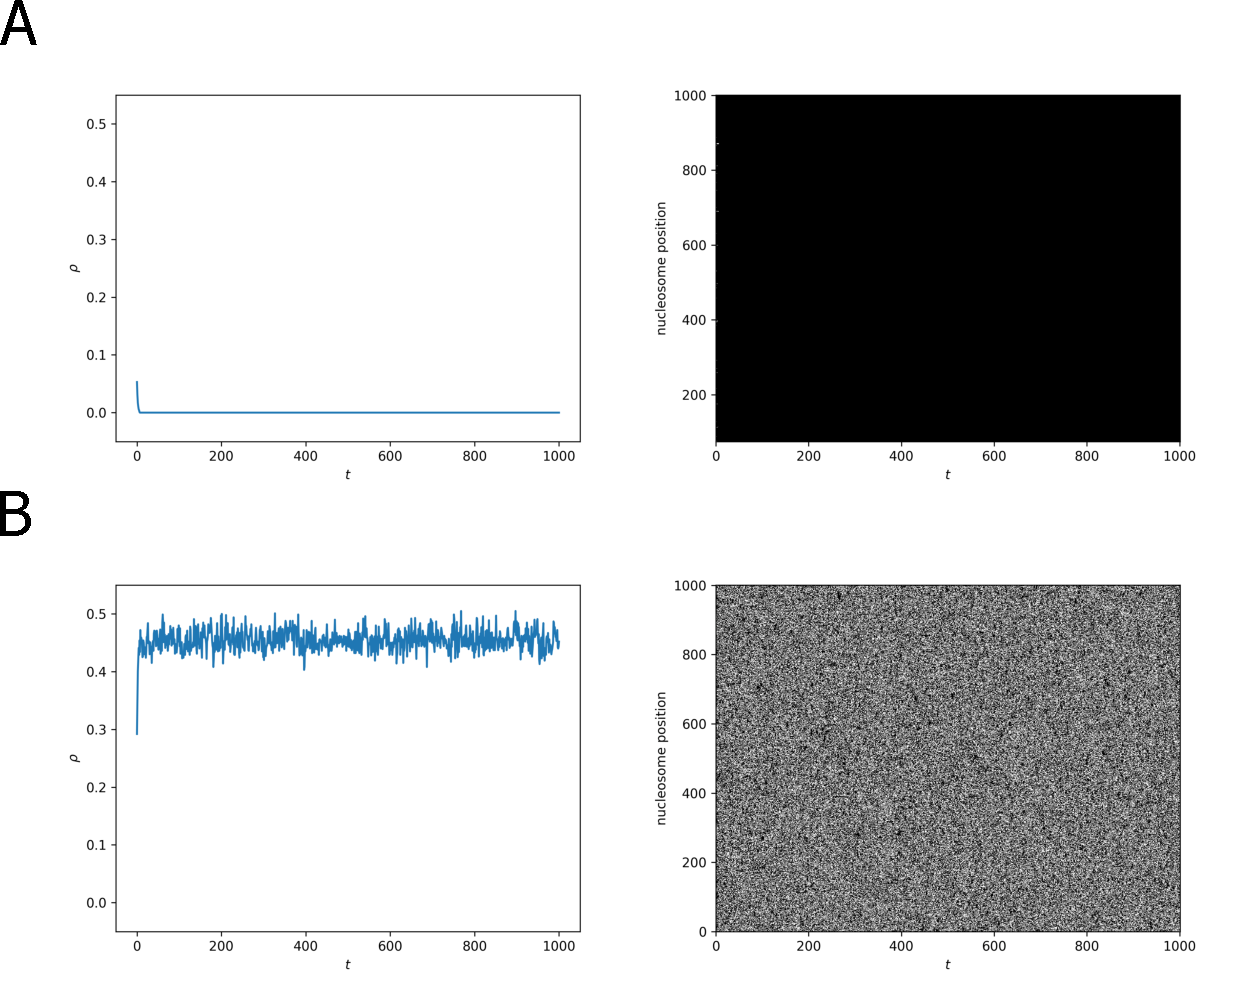
\includegraphics[width=0.9\textwidth]{chapter2/figures/global_coop.pdf}
  \caption[Global cooperative deposition generated bi-stability]{Global cooperative deposition generated bi-stability. The simulations were conducted at $NN$=1000, $\alpha$=1, $\sigma$=3, $rr$=5. (A) The density evolution map and spatial pattern kymographs of the global cooperative deposition model starting from low initial density ($\rho_{0}$=0.05). (B) The density evolution map and spatial pattern kymographs of the global cooperative deposition model starting from high initial density ($\rho_{0}$=0.3).}
  \label{fig:globalCoop}
\end{figure}

\subsection{Arbitrary number control leads to the clustering of CENP-A nucleosomes}

In \textit{Drosophila}, the amount of centromeric CENP-A has been found to negatively correlate with the duration of mitosis, which is when its CENP-A replenishment occurs. Moreover, shortened mitotic time window resulted in decreased centromeric CENP-A level \citep{Pauleau2019TheCells}. This brings the possibility that there might exist self-correcting mechanisms for CENP-A density at the centromere. Hence, we decided to introduce arbitrary number control to our basic model. 

To implement arbitrary number control in simulation, I wanted to set the replenishment strength to be negatively correlated with the number of CENP-A nucleosomes. To this end, I explored two different methods, either changing $\alpha$ or changing $rr$ according to density, and both of them gave similar results. The results of changing $\alpha$ are presented hereafter. In this method, $\alpha$ was described by the following equation (note that the target density $\rho_{target}$ had to be multiplied by two because of the dilution event):
\begin{equation}\label{eq:8}
\begin{split}
        & \alpha = 0 \:\: (\rho > 2\rho_{target}) \\
        & \alpha = 1 - \frac{\rho}{2\rho_{target}} \:\: (\rho \le 2\rho_{target})
\end{split}
\end{equation}
To reflect the real biological system, I set $\rho_{target}$ at 0.02 as suggested in the human cells \citep{Bodor2014}. In mean-field approximation, similar to the basic model, two fixed points existed with the zero one being unstable and the non-zero one being stable. Consistent with our aim, the non-zero fixed point had a value of 0.02 (Figure~\ref{fig:numberControl}A). In the simulation, the density evolution map indicated that arbitrary number control successfully stabilised CENP-A density around the target 0.02. Interestingly, from the kymograph, it can be seen that although multiple islands existed in the first few time steps, only very few, a single one for most of the time, were maintained throughout the simulation (Figure~\ref{fig:numberControl}B and C). We reasoned that this was due to the fact that the total number of CENP-A nucleosomes was limited. The larger island had a higher chance of depositing new CENP-A nucleosomes nearby and therefore grew at the expense of the shrinkage of small ones. Nevertheless, I concluded that arbitrary number control was insufficient to explain the dynamics of the CENP-A system. 

\begin{figure}[htbp]
  \centering
  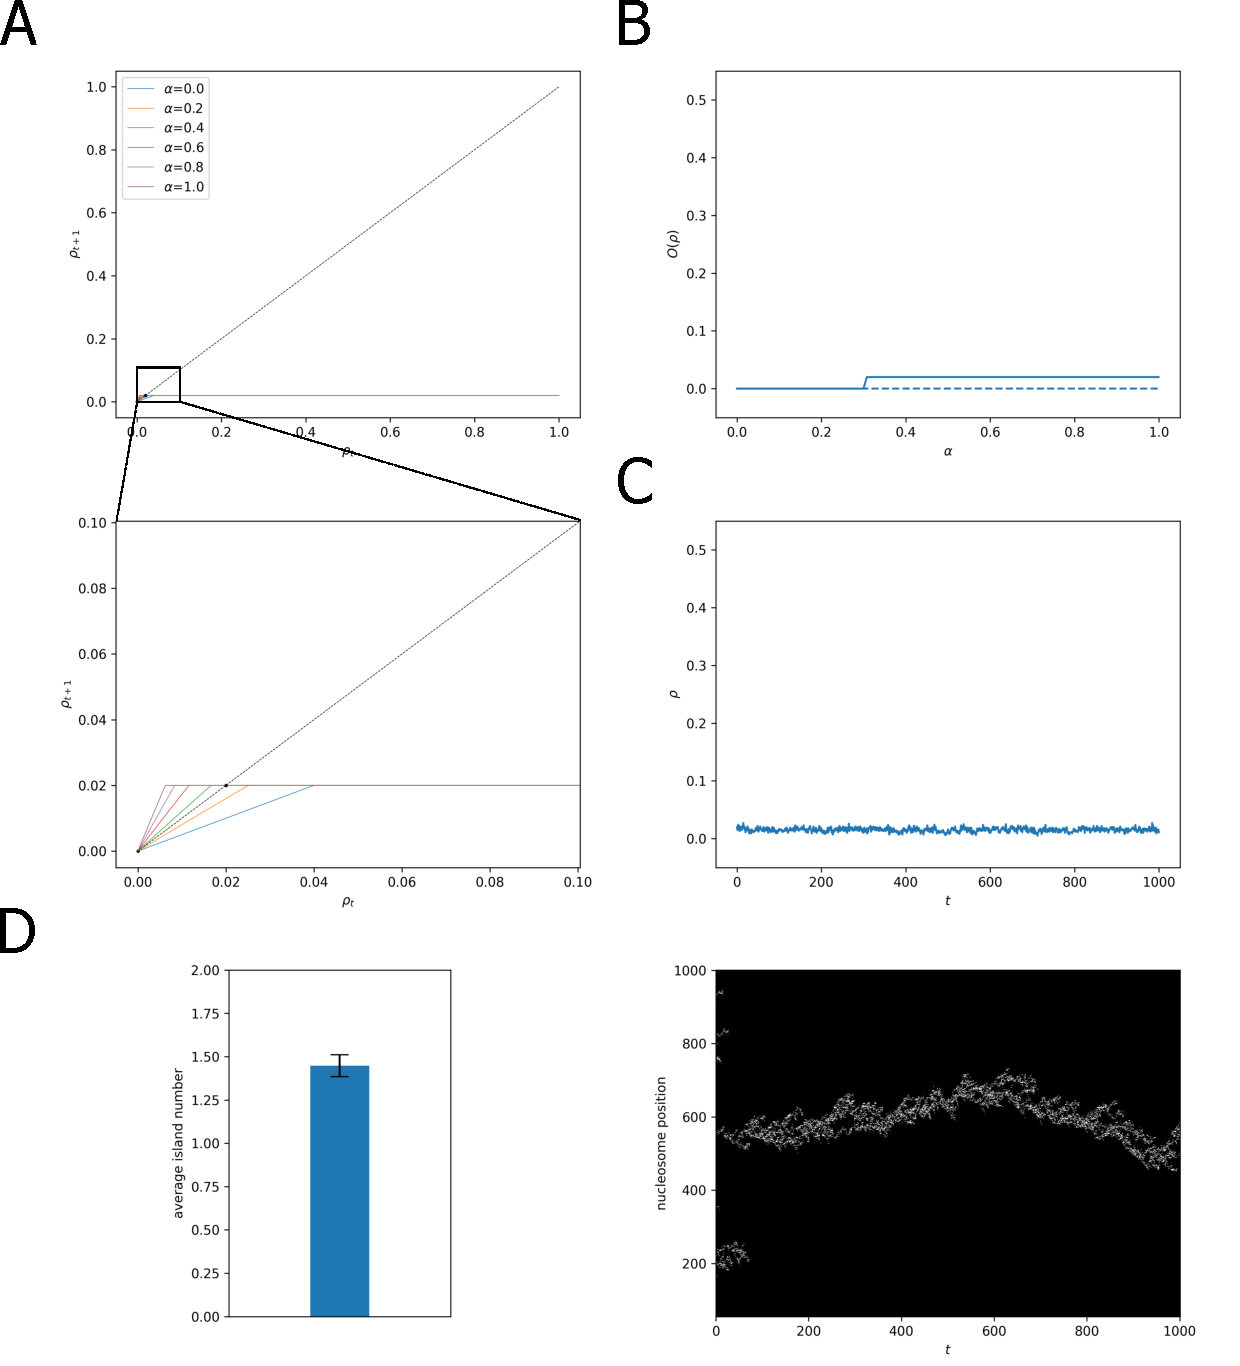
\includegraphics[width=0.9\textwidth]{chapter2/figures/number_conrol.pdf}
  \caption[Arbitrary number control resulted in a pattern of one or two large islands]{Arbitrary number control resulted in a pattern of one or two large islands. (A) Cobweb plot of the arbitrary number control model. The mean-field approximations of the arbitrary number control model with $\rho_{target}$=0.02 were shown. The fixed points were indicated as black dots. The bottom plot is the zoom-in of $\rho{t}$=0-0.1 and $\rho{t+1}$=0-0.1. (B) The density evolution map and spatial pattern kymographs of the arbitrary number control model. The simulations were conducted at $NN$=1000, $\sigma$=3, $rr$=3, $\rho_{0}$=0.02, $\rho_{target}$=0.02. (C) The average number of islands of 10 simulations after 2000 time steps. The error bar represents the standard deviation.}
  \label{fig:numberControl}
\end{figure}

\subsection{Spontaneous conversion can recapitulate the island pattern but not bi-stability}

Due to the fact that CENP-A nucleosomes can also be found on chromosome arms in low density \citep{Bodor2014}, there might exist random incorporation of CENP-A nucleosomes. To test this idea, we decided to explore the spontaneous conversion from canonical H3 nucleosomes to CENP-A nucleosomes in the basic model. A new parameter $\eta$ denoting the rate for this event to happen was introduced (Table~\ref{tab:parametersSpontaneousConversion}). 

\begin{table}[htbp]
\centering
\caption{Additional parameter(s) of the spontaneous conversion model}
\label{tab:parametersSpontaneousConversion}
\begin{tabular}{cl}
\hline
\textbf{Parameters} & \multicolumn{1}{c}{\textbf{Description}} \\ \hline
$\eta$                  & H3 spontaneous conversion rate     \\ \hline
\end{tabular}
\end{table}

As we arbitrarily set the timing of spontaneous conversion to be before dilution and after replenishment, the mean-field approximation then became: 
\begin{equation}\label{eq:9}
\begin{split}
            &\rho_{t+1} = \frac{(1 - \eta)R^{rr}(\rho_{t}) + \eta}{2}\\
            &R(\rho_{t}) = -\omega \rho_{t}^{2} + (1 + \omega) \rho_{t}
\end{split}
\end{equation}
where $\omega = \alpha(1 - f(0))$. 

Intuitively, adding spontaneous conversion into the basic model would rescue the 'dead' type behaviour. To keep the density at a reasonably low value, I chose a parameter set that would have resulted in an asymptotic density of 0 if it were used for the basic model to make the Cobweb plot (Figure~\ref{fig:spontaneousConversion}A). There could only be one fixed but the value is positively correlated with $\eta$ (Figure~\ref{fig:spontaneousConversion}B). As expected, with properly adjusted $\eta$, the densities of the spontaneous conversion model could be maintained around the desired value of 0.02. Importantly, from the spatial pattern kymograph, the island pattern of CENP-A nucleosomes was able to persist throughout the simulation (Figure~\ref{fig:spontaneousConversion}C). However, as shown by the mean-field approximation, the spontaneous conversion model does not possess bi-stability. 

\begin{figure}[htbp]
  \centering
  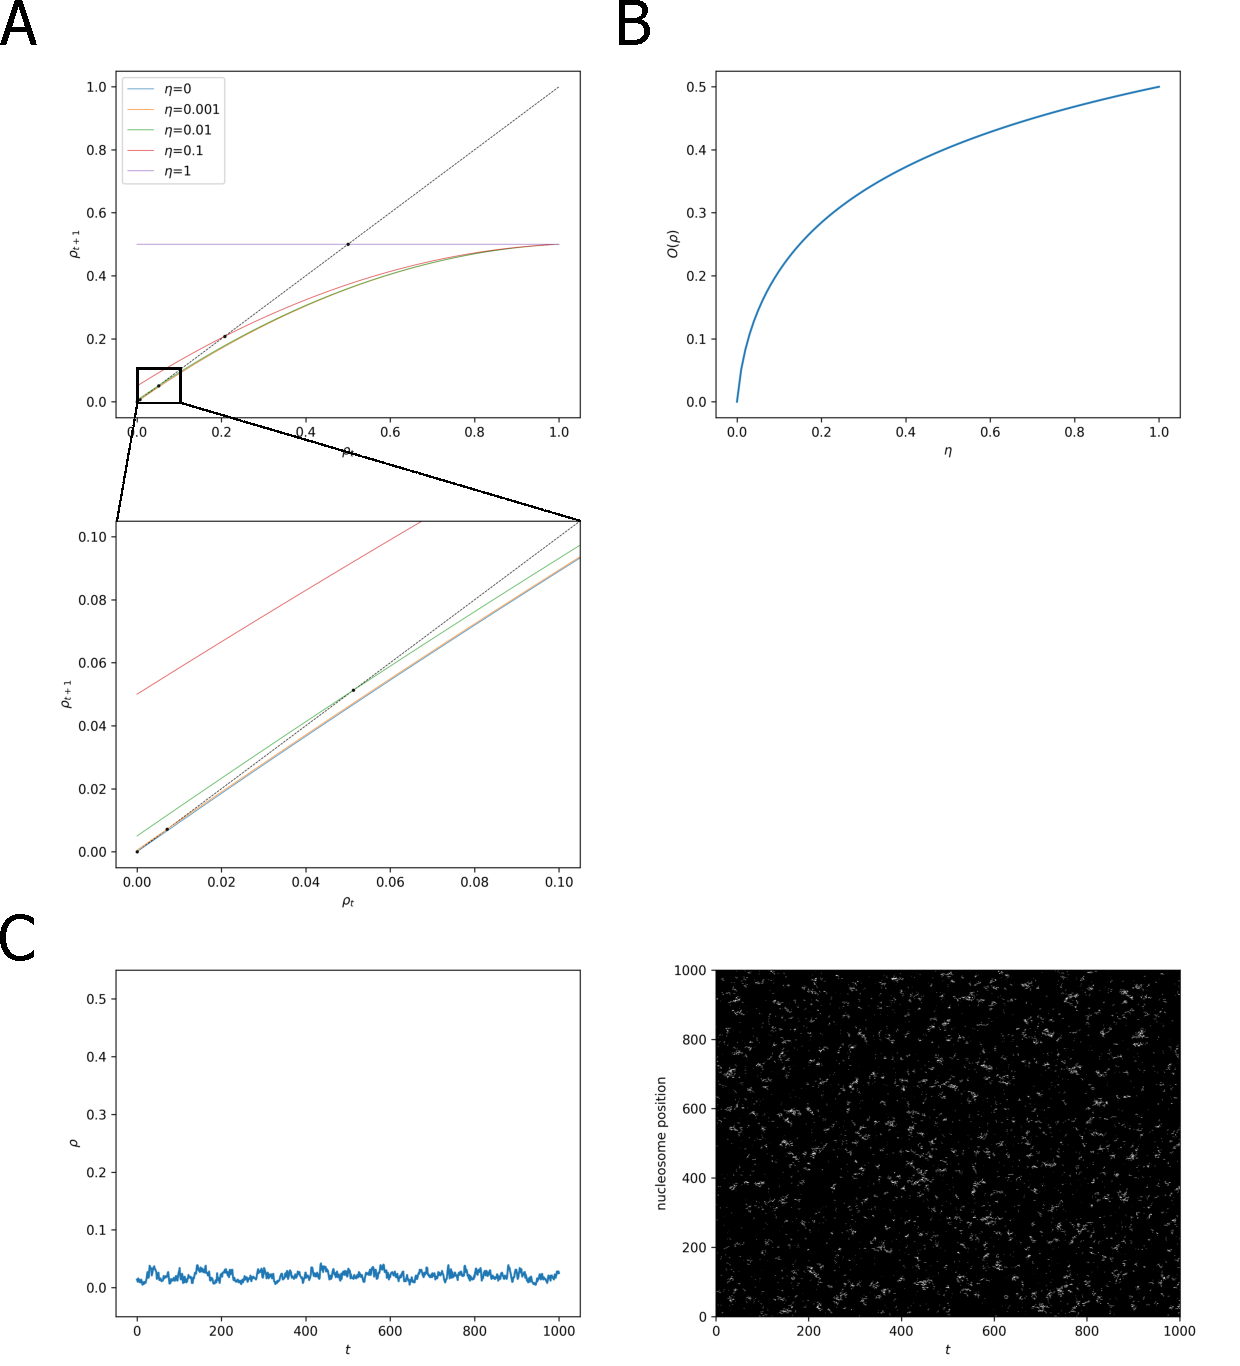
\includegraphics[width=0.9\textwidth]{chapter2/figures/spontaneous_conversion.pdf}
  \caption[Spontaneous conversion was able to maintain the island pattern]{Spontaneous conversion was able to maintain the island pattern. (A) Cobweb plot of the spontaneous conversion model. The mean-field approximations of the spontaneous conversion model with different $\eta$s were shown as coloured curves. The fixed points were indicated as black dots. The bottom plot is the zoom-in of $\rho{t}$=0-0.1 and $\rho{t+1}$=0-0.1. (B) Bifurcation diagram of the spontaneous conversion model. The fixed densities were plotted as a function of $\eta$. The stable branch was shown as the solid line, whereas the unstable one was shown as the dotted line. (C) The density evolution map and spatial pattern kymographs of the spontaneous conversion model. The simulations were conducted at $NN$=1000, $\alpha$=1, $\sigma$=3, $rr$=1, $\rho_{0}$=0.02, $\eta$=0.005.}
  \label{fig:spontaneousConversion}
\end{figure}

\subsection{Adding threshold-based stabilisation to the spontaneous conversion model was able to produce bi-stability, low density and island pattern}

Replication is the major 'sculpting' mechanism through which ectopic CENP-A nucleosomes are actively removed \citep{Nechemia-Arbely2019, Wang2021PhosphorylationCycle}. It has been proposed that CCAN is responsible for the protection of centromeric CENP-A and that its recruitment requires a critical local concentration of CENP-A \citep{Nechemia-Arbely2019, Bodor2014}. This led us to the idea of adding a threshold-based stabilisation mechanism to our model. Given the success of the spontaneous conversion model in recapitulating the low density and island pattern, I decided to introduce threshold-based stabilisation to the spontaneous conversion model. Specifically, I set an arbitrary value that any density below would be returned to zero. 

As expected, introducing threshold-based stabilisation was able to create two stable fixed points on the Cobweb plot, indicating the potential to generate bi-stability (Figure~\ref{fig:doubleCobweb}A). Indeed. by simulating the model, two stably inherited states were observed from the density evolution map and spatial distribution kymograph, one with a lower density and more scattered CENP-A nucleosomes while the other one with a higher density and a more clustered distribution (Figure~\ref{fig:doubleCobweb}B). However, the two states inter-converted spontaneously with the parameter set tested, which is in contrast to the experimental data that neo-centromeres are rare \citep{Marshall2008Neocentromeres:Evolution}. 

\begin{figure}[htbp]
  \centering
  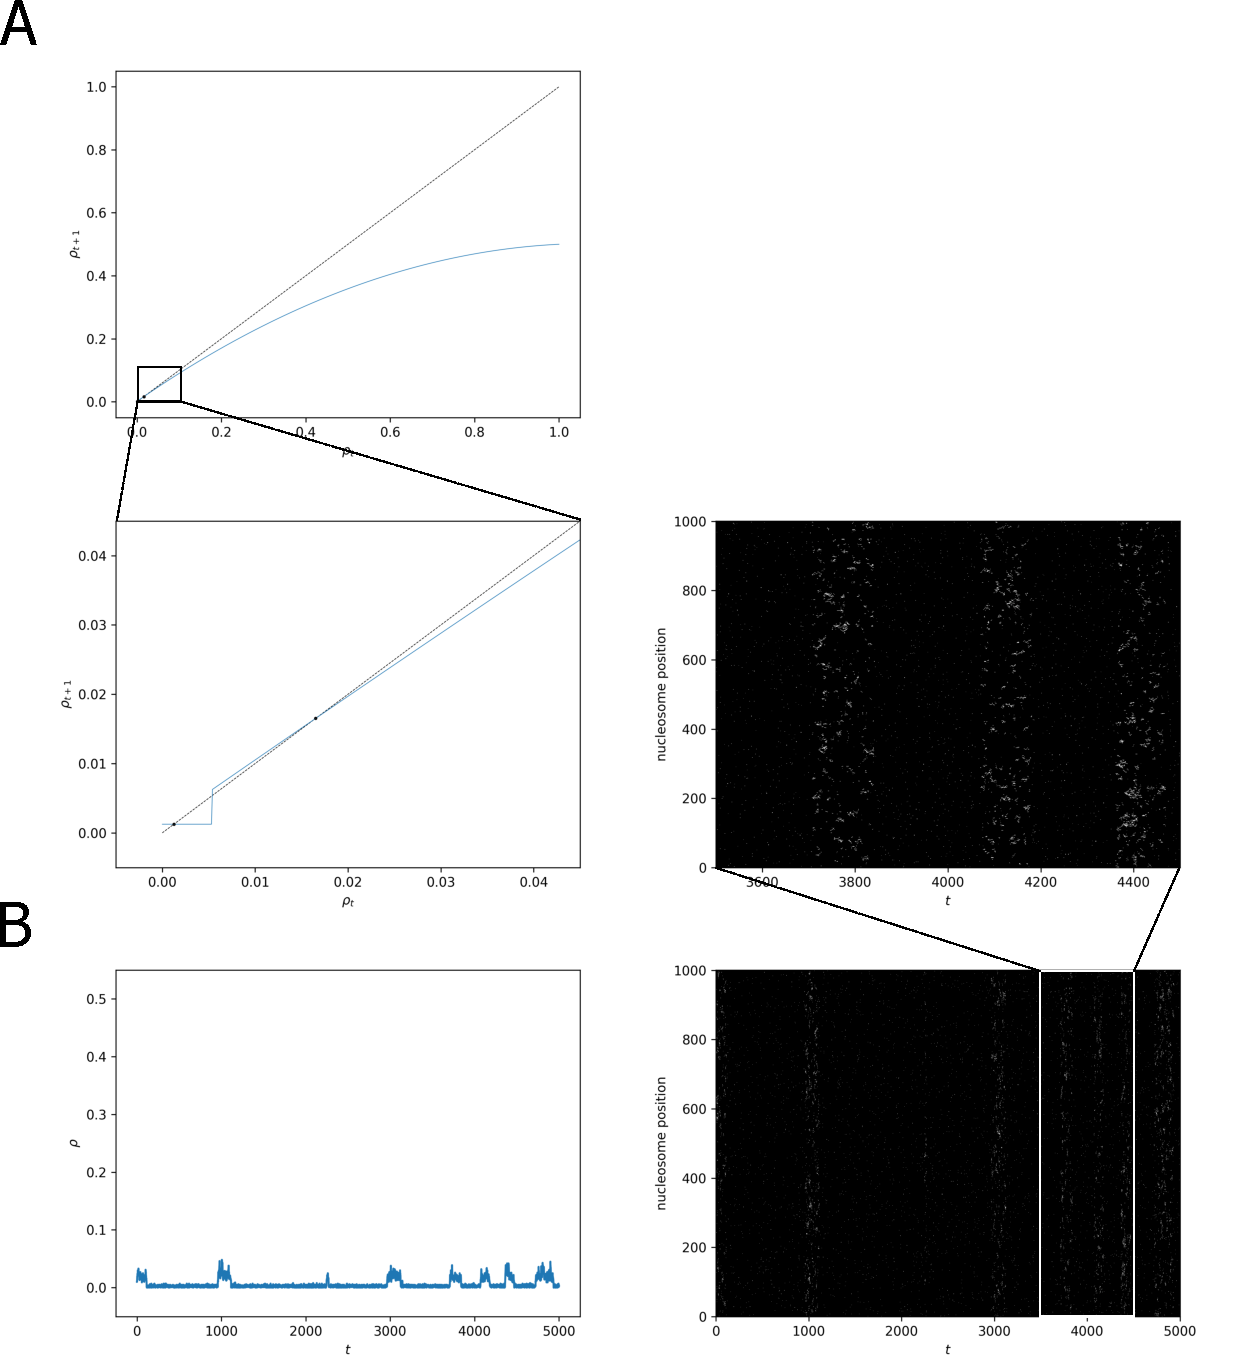
\includegraphics[width=0.9\textwidth]{chapter2/figures/doubleCobweb.pdf}
  \caption[Adding threshold-based stabilisation to the spontaneous conversion model generated bi-stability but the steady states inter-converted spontaneously]{Adding threshold-based stabilisation to the spontaneous conversion model generated bi-stability but the steady states inter-converted spontaneously. (A) Cobweb plot of the threshold-based stabilisation model. The mean-field approximations of the threshold-based stabilisation model with $\alpha$=1, $\sigma$=3, $rr$=1, $\eta$=0.0025, sculpting threshold=0.0075 were shown. The fixed points were indicated as black dots. The bottom plot is the zoom-in of $\rho{t}$=0-0.1 and $\rho{t+1}$=0-0.1. (B) The density evolution map and spatial pattern kymographs of the threshold-based stabilisation model. The upper plot is the zoom-in of the white box in the lower plot. The simulations were conducted at $NN$=1000, $\alpha$=1, $\sigma$=3, $rr$=1, $\eta$=0.0025, sculpting threshold=0.0075. }
  \label{fig:doubleCobweb}
\end{figure}

To reduce the stochasticity of the system, one possible method is to increase the size $NN$, as shown in Figure~\ref{fig:parameterTest}B. After changing $NN$ from 1000 to 5000, which is the average nucleosome number of human cells \citep{Bodor2014}, the threshold-based stabilisation model exhibited robust inheritance of the two states (Figure~\ref{fig:doubleLongArray}A and B). Therefore, I concluded that adding threshold-based stabilisation to the spontaneous conversion model was able to recapitulate the three goals of the CENP-A model, namely bi-stability, low density at the higher steady state and the maintenance of island patterns.


\begin{figure}[htbp]
  \centering
  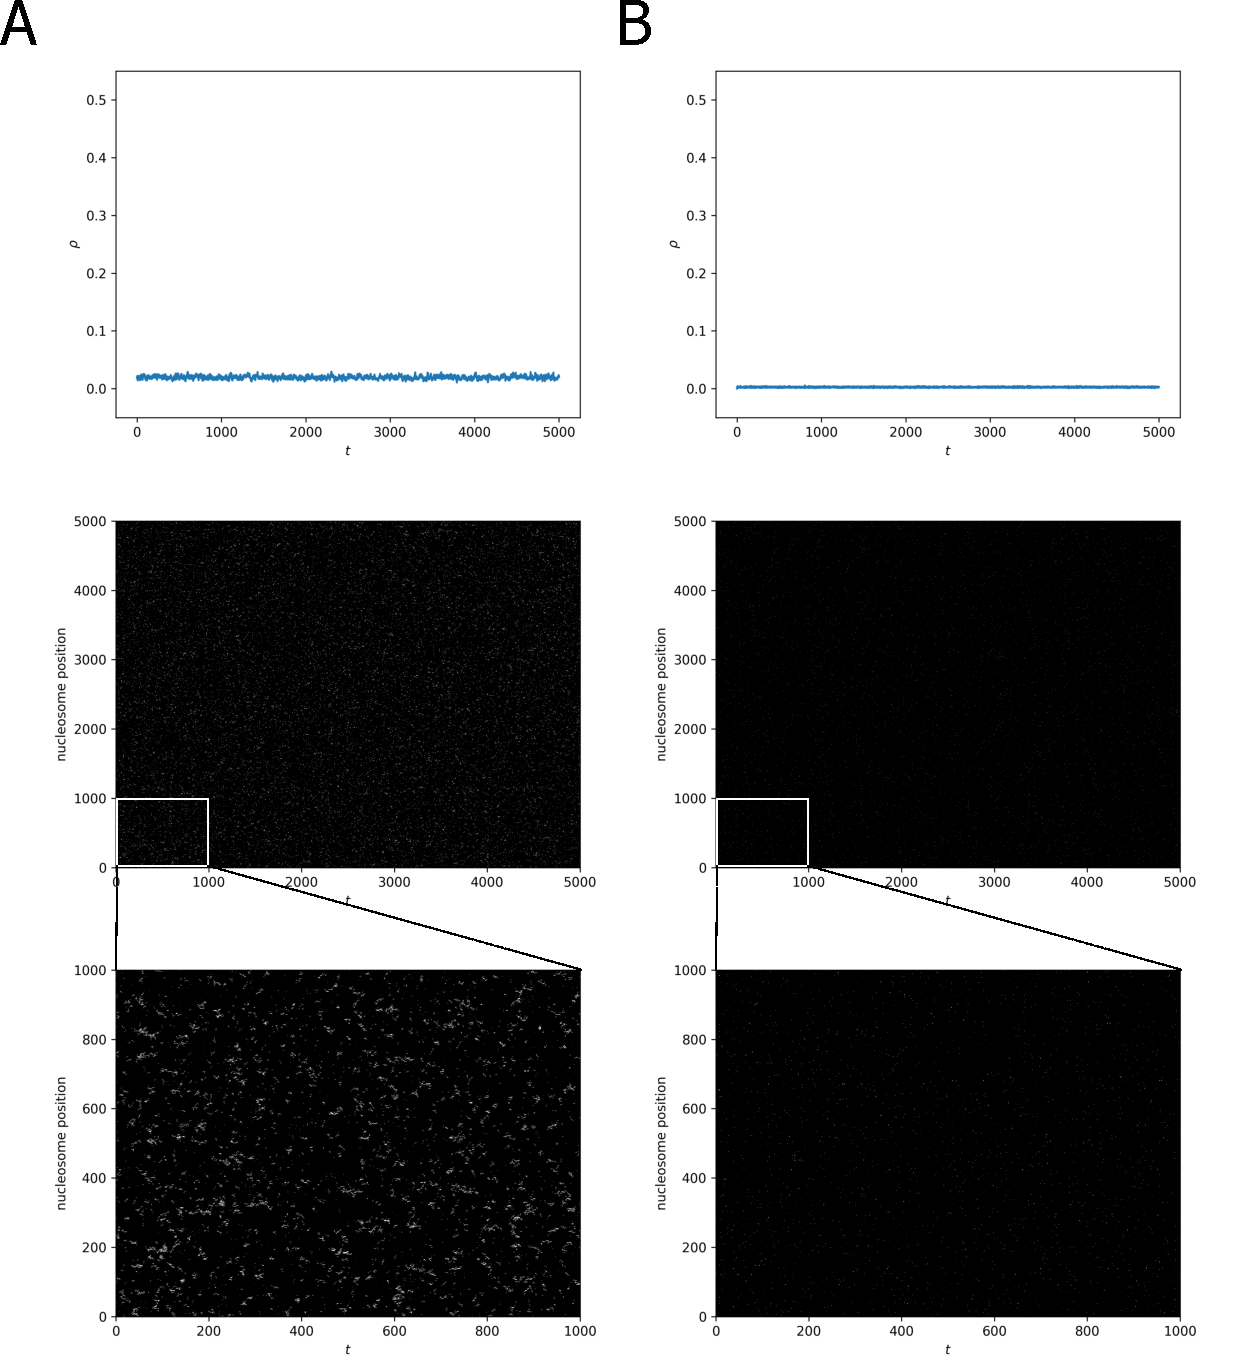
\includegraphics[width=0.9\textwidth]{chapter2/figures/doubleLongArray.pdf}
  \caption[Increasing $NN$ stabilised the steady states]{Increasing $NN$ stabilised the steady states. The simulations were conducted at $NN$=5000, $\alpha$=1, $\sigma$=3, $rr$=1, $\eta$=0.0025, sculpting threshold=0.0075. (A) The density evolution map and spatial pattern kymographs of the threshold-based stabilisation model starting from high initial density ($\rho_{0}$=0.02). The bottom plot is the zoom-in of the white box in the upper plot. (B) The density evolution map and spatial pattern kymographs of the threshold-based stabilisation model starting from low initial density ($\rho_{0}$=0). The bottom plot is the zoom-in of the white box in the upper plot.}
  \label{fig:doubleLongArray}
\end{figure}

\section{Discussion}

With the aim of recapitulating the three key characteristics of the establishment and maintenance of CENP-A nucleosomes, that is bi-stability, low density and island pattern, we started with a simplified rule-based CA-like model named the basic model. The basic model is a 1D string of either CENP-A or H3 nucleosomes. The update of such a model consisted of replenishment, where new CENP-A nucleosomes were incorporated locally with positive feedback, and dilution, where around half of the CENP-A were lost. The basic model failed to meet the characteristics we wanted to model. Hence, we explored different possible mechanisms and tested if they can change the model behaviours towards the goals set. The mechanisms and their outcomes are summarised in Table~\ref{tab:summary}. 

\begin{table}[htbp]
\centering
\caption{Summary of the behaviours of models tested}
\label{tab:summary}
\begin{tabular}{lccc}
\hline
\multicolumn{1}{c}{\textbf{Model}}                        & \textbf{Bi-stability}   & \textbf{Low density} & \textbf{Island pattern} \\ \hline
1. Basic                                                     & \ding{55} &          \ding{55}            &         \ding{55}                \\
2. Global   cooperative deposition                                    &  \ding{51}                       &        \ding{55}              &           \ding{55}              \\
3. Arbitrary number   control                                          &          \ding{55}               &           \ding{51}           &      \ding{55}                   \\
4. Spontaneous   conversion                                  &          \ding{55}               &          \ding{51}            &    \ding{51}                     \\
\begin{tabular}[c]{@{}l@{}}5. Threshold-base stabilisation \\ \;\;\;\;+ spontaneous conversion\end{tabular} &           \ding{51}              &           \ding{51}           &        \ding{51}                 \\ \hline
\end{tabular}
\end{table}

\subsection{The basic model}

Both the simulations and analytical methods suggested that the basic model has two possible behaviours depending on the parameters. One where CENP-A nucleosomes can form islands temporarily but lose them eventually and one where CENP-A nucleosomes quickly saturate the available space and stay in this state (Figure~\ref{fig:modelBehaviour}). Apparently, neither of the two behaviours resembled the experimental data on CENP-A dynamics. Despite that, Several implications could be drawn from the results. First, the mechanism of local deposition with positive feedback is capable of supporting the formation of the island pattern, although the maintenance of such a pattern needs additional help. Second, due to the nature of positive feedback, the density of CENP-A nucleosomes could only be at two extremes, either zero or near saturation. Third, the positive feedback alone is insufficient to give rise to bi-stability, consistent with previous conclusions \citep{Lewis1977ThresholdsDevelopment, Thomas2001MultistationarityBehavior, Ferrell2002Self-perpetuatingBistability, Smits2006PhenotypicRegulation., Dodd2007}. 

\subsection{The global cooperative deposition model}

\cite{Dodd2017} suggested that bi-stability in a 1D epigenetics model requires three elements, namely positive feedback, cooperativity and beyond-local interactions. Therefore, I implemented global cooperative deposition in the basic model to obtain bi-stability in our model. Indeed, the model was able to exhibit two distinct steady states with the same set of parameters, both analytically (Figure~\ref{fig:coopSchematics}) and numerically (figure~\ref{fig:globalCoop}). However, the densities of CENP-A nucleosomes of the 'high' state were over a magnitude higher than what was observed in biological systems. This indicated that the classical mechanistic explanation for bi-stability might not underlie the CENP-A system. Alternatively, it is possible that CENP-A nucleosomes cluster and induce centromere higher-order structure \textit{in vivo}, which had recently been supported both experimentally \citep{Zhou2022, Andronov2019} and theoretically \citep{Camara2021ASpecies}, raising the effective local density to a level that the cooperative deposition model could describe. Molecular dynamics simulation methods could be used to test this possibility. 

\subsection{The arbitrary number control model}

Experimental data from \textit{Drosophila} indicated there might exist an active self-correcting mechanism to maintain the number of centromeric CENP-A nucleosomes at homeostasis \citep{Pauleau2019TheCells}. To test the hypothesis, I implemented arbitrary number control in the basic model (Figure~\ref{fig:numberControl}). In this model, the density of CENP-A nucleosomes was able to be maintained around the desired values as expected. However, the CENP-A nucleosomes were concentrated and formed one or two large islands instead of a few as shown in extended chromatin experiments \citep{Blower2002ConservedHumans, Dunleavy2011H3.3Phase., Kyriacou2018}, suggesting active monitoring of centromeric CENP-A density is unlikely. Interestingly, this result is in striking consistency with the established conclusion from the cell polarity determination research that auto-catalytic reaction and mass conservation eventually lead to the formation of a single maximum \citep{Goryachev2020CompeteOutcomes, Goehring2012OrganelleComponents, Otsuji2007APolarity}.

\subsection{The spontaneous conversion model}

Random deposition of CENP-A into chromatin has been supported by different experimental observations. Ectopic CENP-A nucleosomes account for the major portion of chromatin-incorporated CENP-A \citep{Bodor2014}. Overexpression of CENP-A greatly increased its mislocation \citep{Gascoigne2011, VanHooser2001SpecificationCENP-A}. To explore if this mechanism could alter the behaviours of our model, I added the random conversion from H3 nucleosomes to CENP-A nucleosomes to the basic model (Figure~\ref{fig:spontaneousConversion}). Although could not create bi-stability, this model was able to recapitulate both the low density and island patterns characteristics of the system. We reasoned that this is because the random conversion rescued the 'dead' type behaviour of the basic model by enabling the emergence of new islands. Along the same line, any mechanism introducing beyond-local deposition weaker than the local deposition of CENP-A could generate such behaviour. So far, I have tested introducing weak long-range deposition in the known positive feedback loop and it showed a similar outcome as the spontaneous conversion model. 

\subsection{The threshold-based stabilisation and spontaneous conversion model}

Various methods are adopted by the cells to sculpt CENP-A distribution via evicting ectopic CENP-A nucleosomes \citep{Stirpe2022}. CCAN has been indicated to spare the centromeric CENP-A from sculpting \citep{Nechemia-Arbely2019}. Also, it has been proposed that a critical density of CENP-A nucleosomes is required for kinetochore formation \citep{Bodor2014}. Together, they suggested a threshold-based stabilisation mechanism, which could potentially generate bi-stability. To test this possibility, I implemented threshold-based stabilisation in the spontaneous conversion model (Figure~\ref{fig:doubleCobweb}), given the desired behaviours it provided. Indeed, this model did show bi-stability and could recapitulate all the three characteristics we aimed for. For the model to be true, it is important to first experimentally verify the assumption that the formation of kinetochore does require a critical number of CENP-A nucleosomes within a certain range of chromatin. Besides, the model requires this value to be higher than the level of random CENP-A incorporation, which is estimated to be about \num{8e-4} \citep{Bodor2014}. It would be informational to compare the two numbers. It was also found in the simulation that the robustness of steady states depends on the total number of nucleosomes modelled. This predicted that the chromosome with a shorter centromere would have a higher chance of neo-centromere formation. It would be interesting to test whether it is the case in real biological systems. 
